\documentclass[review]{elsarticle}
\usepackage{amsmath}
\usepackage{lineno,hyperref}
\usepackage[left=2cm, right=2cm, top=3cm, bottom=3cm]{geometry}
\usepackage{booktabs}
\usepackage{makecell}
\usepackage{tabularx}
\usepackage{amssymb}
\usepackage{array,caption,threeparttable}
\usepackage[font=small,labelfont=bf,labelsep=none]{caption}
\usepackage{graphicx}
\usepackage{epstopdf}
\usepackage{tikz}
\usepackage{verbatim}
\usepackage{cleveref}
\hypersetup{
    colorlinks=true, % 允许超链接使用颜色
    linkcolor=blue,  % 图片引用链接颜色
}

\usetikzlibrary{matrix, positioning}
\modulolinenumbers[5]

\crefname{figure}{Fig.}{Figs.}
\crefname{table}{Table}{Table}
\newcommand{\figref}[1]{\hyperref[#1]{Fig.~\ref*{#1}}}
\newcommand{\tabref}[1]{\hyperref[#1]{Table~\ref*{#1}}}
\journal{Journal of \LaTeX\ Templates}

%%%%%%%%%%%%%%%%%%%%%%%
%% Elsevier bibliography styles
%%%%%%%%%%%%%%%%%%%%%%%
%% To change the style, put a % in front of the second line of the current style and
%% remove the % from the second line of the style you would like to use.
%%%%%%%%%%%%%%%%%%%%%%%

%% Numbered
%\bibliographystyle{model1-num-names}

%% Numbered without titles
%\bibliographystyle{model1a-num-names}

%% Harvard
%\bibliographystyle{model2-names.bst}\biboptions{authoryear}

%% Vancouver numbered
%\usepackage{numcompress}\bibliographystyle{model3-num-names}

%% Vancouver name/year
%\usepackage{numcompress}\bibliographystyle{model4-names}\biboptions{authoryear}

%% APA style
%\bibliographystyle{model5-names}\biboptions{authoryear}

%% AMA style
%\usepackage{numcompress}\bibliographystyle{model6-num-names}

%% `Elsevier LaTeX' style
\bibliographystyle{elsarticle-num}
%%%%%%%%%%%%%%%%%%%%%%%


\captionsetup[table]{
labelsep=newline,
singlelinecheck=false,
}
\captionsetup[figure]{name={Fig.},labelsep=period}
\begin{document}

\begin{frontmatter}

\title{Elsevier \LaTeX\ template\tnoteref{mytitlenote}}
\tnotetext[mytitlenote]{Fully documented templates are available in the elsarticle package on \href{http://www.ctan.org/tex-archive/macros/latex/contrib/elsarticle}{CTAN}.}

%% Group authors per affiliation:
\author{Elsevier\fnref{myfootnote}}
\address{Radarweg 29, Amsterdam}
\fntext[myfootnote]{Since 1880.}

%% or include affiliations in footnotes:
\author[mymainaddress,mysecondaryaddress]{Elsevier Inc}
\ead[url]{www.elsevier.com}

\author[mysecondaryaddress]{Global Customer Service\corref{mycorrespondingauthor}}
\cortext[mycorrespondingauthor]{Corresponding author}
\ead{support@elsevier.com}

\address[mymainaddress]{1600 John F Kennedy Boulevard, Philadelphia}
\address[mysecondaryaddress]{360 Park Avenue South, New York}

\begin{abstract}
This template helps you to create a properly formatted \LaTeX\ manuscript.
\end{abstract}

\begin{keyword}
\texttt{elsarticle.cls}\sep \LaTeX\sep Elsevier \sep template
\MSC[2010] 00-01\sep  99-00
\end{keyword}

\end{frontmatter}

\linenumbers

\section{The Elsevier article class}

\paragraph{Installation} If the document class \emph{elsarticle} is not available on your computer, you can download and install the system package \emph{texlive-publishers} (Linux) or install the \LaTeX\ package \emph{elsarticle} using the package manager of your \TeX\ installation, which is typically \TeX\ Live or Mik\TeX.

\paragraph{Usage} Once the package is properly installed, you can use the document class \emph{elsarticle} to create a manuscript. Please make sure that your manuscript follows the guidelines in the Guide for Authors of the relevant journal. It is not necessary to typeset your manuscript in exactly the same way as an article, unless you are submitting to a camera-ready copy (CRC) journal.

\paragraph{Functionality} The Elsevier article class is based on the standard article class and supports almost all of the functionality of that class. In addition, it features commands and options to format the
\begin{itemize}
\item document style
\item baselineskip
\item front matter
\item keywords and MSC codes
\item theorems, definitions and proofs
\item lables of enumerations
\item citation style and labeling.
\end{itemize}

\section{Description of RKC method }
\subsection{Classic one-step RKC methons}
Let $y_n$ represent the approximation to the exact solution $y(n)$ at time $t=t_n$ and $h=t_{n+1}-t_n$ 
is the time step size. For the ODE system(1),the formulas of one-step RKC method with s stage can be defined as 
\begin{align}
    & K_{0}=y_{n},\nonumber \\
    &K_{1}=y_{n}+\tilde{u}_{1}hF_{0}, \nonumber\\
    &K_{j}=u_{j}K_{j-1}+v_{j}K_{j-2}+(1-u_{j}-v_{j})K_{0}+\tilde{u}_{j}hF_{j-1}+\tilde{\gamma}_{j}hF_{0},\quad j\geq2, \nonumber\\
    &y_{n+1}=K_{s},\quad n=0,1,\ldots,N-1, \nonumber
\end{align}
where \(F_j = f(t_n + c_jh, K_j)\),and $y_0=y(t_0)$, the coefficients \(u_j, v_j, \tilde{u}_j, \tilde{v}_j, \tilde{\gamma}_j \in R \),
 $c_j$ has the following recursive format,
\begin{align}
    &c_0=0,c_1=+\tilde{u_1},\nonumber\\
    &c_j = u_j c_{j-1} + v_j c_{j-2} + \tilde{u}_j + \tilde{\gamma}_j, \quad 2 \leq j \leq s. \nonumber
\end{align}

Based on [],if the correlation coefficients satisfy the following conditions, 
then the RKC method has second-order accuracy
\begin{align}
    &\tilde{u}_{1} =b_{1} ,\quad \omega_{1}=\frac{T_{s}^{\prime}\quad(\omega_{0})}{T_{s}^{\prime\prime}(\omega_{0})}, \quad  \omega_{0}=1+\frac{\eta}{s^{2}}, \quad b_{0}=b_{1}=b_{2},\nonumber  \\
    &u_{j} =2\omega_{0}\frac{b_{j}}{b_{j-1}},\quad v_{j}=-\frac{b_{j}}{b_{j-2}},\quad\tilde{u}_{j}=2\omega_{1}\frac{b_{j}}{b_{j-1}}, \nonumber \\
    &\tilde{\gamma}_{j} =-\big(1-b_{j-1}T_{j-1}(\omega_{0})\big)\tilde{u}_{j},\quad b_{j}=\frac{T_{j}^{\prime\prime}(\omega_{0})}{\big(T_{j}^{\prime}(\omega_{0})\big)^{2}},\quad2\leq j\leq s, \nonumber
\end{align}

Here, $\eta \geq 0$ is a small free damping parameter, and changing the value of $\eta$ typically alters the shape of the stability region,
for the second-order RKC method, $\eta = \frac{2}{13}$ is an appropriate value to use.

Apply the second-order RKC method to the test problem (), and the expression for the second-order consistent stability function is as follows:
$$
P_s(z)=1-b_sT_s(\omega_0)+b_sT_s(\omega_0+\omega_1z)
$$
where $a_{j}=1-b_{j}T_{j}(\omega_{0}).$

The stabilisation domain of the RKC method is usually a narrow region around the negative real axis, whose length is proportional to $s^2$
,for the second-order method described above, the real stabilisation interval is $[-0.65s^2,0]$ , and the optimal parameters can be chosen so that the length of the negative real-axis interval reaches approximately $0.81s^2$, as described in $[]$.

\subsection{The two-step RKC method}

The two-step RKC method was devised by B.P. Sommeijer et al [111]. in 2007, which has a similar formulation to the multi-step method, assuming that $y_{n-1},y_{n}$ are the numerical solutions obtained from the two-step RKC computed in times $t_{n-1},t_{n}$
.It is represented by the formula:
$$
y_{n+1}=\alpha_{-1}y_{n-1}+\alpha_{0}y_{n}+\alpha\tilde{y_{n+\theta}},
$$

We first apply the RKC formula (11)at $t=t_{n}$,with a starting value of $y_{n}$ and a step size of $\theta h_n$, compute the result obtained in one step, denoted as $y_{n+\theta}$,
and then obtain the new value $\tilde{y_{n+1}}$ by the two-step RKC formula, where $y_{n-1},y_{n}$ are known. The two-step method requires only one more store than the one-step method, 
but gains considerable flexibility in the value of $\omega_{1}$, i.e., a suitable value of $\omega_{1}$ can greatly increase the length of the stability domain around the negative real axis.
For the starting step, one step is computed with the one-step RKC method to obtain an additional starting value, and from the second step onwards, the two-step RKC method is used.

The new parameters $\alpha_{-1}, \alpha_{0}, \alpha \in R $ are used to control the convergence order of the two-step methods. To be precise, we compute the Taylor expansion of $\tilde{y}_{n+\theta}$ and $y_{n-1}$.
\begin{align}
    &\tilde{y}_{n+\theta}=y_n+\theta\tau_ny_n^{\prime}+\frac12\theta^2\tau_n^2y_n^{\prime\prime}+\frac16c\theta^3\tau_n^3y_n^{\prime\prime\prime}+\mathcal{O}(\tau_n^4),\quad c=\frac{T_s^{\prime}(\omega_0)T_s^{\prime\prime\prime}(\omega_0)}{T_s^{\prime\prime}(\omega_0)^2},\nonumber\\
    &{y}_{n-1}=y_n-\tau_{n-1}y^{\prime}+\frac12\tau_{n-1}^2y_n^{\prime\prime}-\frac16\tau_{n-1}^3y_n^{\prime\prime\prime}+\mathcal{O}(\tau_n^4)\nonumber
 \end{align}

Comparison of these formulas with the Taylor expansion of the true solution, the two-step RKC method converges thrid order for linear problems $W^{prime}=AW$if the conditions
\begin{align}
 &\alpha_0 = 1 - \alpha_{-1} - \alpha_{\theta}, \quad \alpha_{\theta} = \frac{1 + r_n}{\theta(1 + \theta r_n)}, \quad \alpha_{-1} = \frac{r_n^2(1 - \theta)}{1 + \theta r_n},(2.2.1)\nonumber\\
 &(cr_{n})\theta^{2}+(1-r_{n})\theta-1=0,(2.2.2)\nonumber
\end{align}
where $r_n=\frac{\tau_n}{\tau_{n-1}}$ is the step ratio,equation(2.2.1) always has two real roots for $\theta$,one of which is negative. Naturally, we require the positive root.
Notably, $s>3$ and $1<\theta<2$ are necessary conditions .If the parameters $\alpha_{-1}, \alpha_{0}, \alpha $ just satisfy the condition(2.2.1), then method (2.2) has second-order consistency for the nonlinear problem
We consider two-step methods with a constant step size that maintain third-order consistency. It is then $\theta = \frac{1}{c}$, insert $y_j=\zeta^j$ into (2.2). This leads to the corresponding characteristic equation:
We consider two-step methods with a constant step size that maintain third-order consistency. It is then $\theta = \frac{1}{c}$, insert $y_j=\zeta^j$ into (2.2). This leads to the corresponding characteristic equation:
$$
\zeta^2 - (\alpha_0 + \alpha_\eta P_s(\theta z))\zeta - \alpha_{-1} = 0 \quad (2.2.3)
$$

The stability regions are determined through numerical construction based on the root condition. Let $\tilde{\beta(s)}$ donate the real stability boundary,similar to the one-step RKC method, 
the value of the damping parameter $\varepsilon$ adjustment can also change the shape of the stabilization domain, and suitable values of $\varepsilon$ have been found(see table 1). For more details, refer to [].



\section{The new two-step RKC formula}

Assume that $y_{n-1},y_n$ are the numerical solutions obtained from the new two-step RKC method at times $t_{n-1},t_n$, and $\tilde{y}_{n-1},\tilde{y}_n$ are obtained by applying a one-step method (e.g., (2.1)) to $y_{n-1},y_n$ with step sizes $\tau_{n-1}$ and $\tau_n$, respectively.
The new two-step method then determines the approximation $y_{n+1}$ at the future time level $t_{n+1}$ as follows:

$$
y_{n+1} = \alpha_{-1}y_{n-1} + \tilde{\alpha}_{-1}\tilde{y}_{n-1} + \alpha_0y_n + \alpha\tilde{y}_n,
$$

By adding new coefficients $\tilde{\alpha_{-1}}$ and storing more of the results from the previous one-step RKC calculation, the computational cost is almost unchanged compared to the two-step RKC, 
but because of $\tilde{\alpha_{-1}}$, we gain additional tuning space for $\omega_{1}$, so the coefficients $\varepsilon,\omega_{0},\omega_{1} $of NTRKC are a bit different from those of the one-step RKC method. 
For NTRKC, the change of damping parameter $\varepsilon$ and $\omega_{1}$ will adjust the shape of the stabilizing domain, the relatively large $\varepsilon$ and $\omega_{1}$ will sacrifice the length of the stabilizing domain for the width,
 and the relatively small $\varepsilon$ and $\omega_{1}$ will get the long but narrow stabilizing domain, NTRKC will have better stabilizing domain than the two-step RKC and also higher numerical accuracy, 
 in the stabilizing domain analysis in the following section, we will elaborate on this, and two sets of coefficients will be given. Selection scheme.

\subsection{Convergence Analysis}
The parameters$ \alpha_{-1},\tilde{\alpha_{-1},\alpha_{0},\alpha} \in R$ are used to control the convergence order of the methods.
Based on [1],Explict Runge-Kutta method (2.1) can be written in a matrix-like format
\begin{figure}[h]
    \centering
    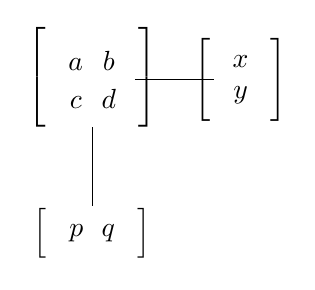
\begin{tikzpicture}
        % Create matrices
        \matrix (mat) [matrix of math nodes, left delimiter={[}, right delimiter={]}]
        {
            a & b \\
            c & d \\
        };

        \matrix (colvec) [right=1cm of mat, matrix of math nodes, left delimiter={[}, right delimiter={]}]
        {
            x \\
            y \\
        };

        \matrix (rowvec) [below=1cm of mat, matrix of math nodes, left delimiter={[}, right delimiter={]}]
        {
            p & q \\
        };

        % Draw lines to separate them
        \draw (mat.east) -- (colvec.west);
        \draw (mat.south) -- (rowvec.north);
    \end{tikzpicture}
\end{figure}


 Let $y_{n-1},y_{n}$ denote approximations to $ y(t_n),y(t_{n-1})$.Fixing the time step $\tau_{n}=\tau$,$\tilde{y_{n-1}}$ has the following estimator due to the change in $\omega_{1}$

 \begin{equation}
    \tilde{y}_{n-1} = y_{n-1} + A_1\tau f_{n-1} + A_2\tau^2f'f_{n-1} + A_3\tau^3f'f'f_{n-1} + A_4\tau^3f''f^2_{n-1} + \mathcal{O}(\tau^4) (3.1.1)\nonumber
\end{equation}
where $f_{n-1}=f(y_{n-1})$,$ \tilde{y_{n-1}},\tilde{y_n}$ are both obtained by the method(2.1), therefore $y_n$ has the same coefficients of the estimator.Considering $f_{n-1}$ as  function with respect to $\tau$,it is readily verified that 
\begin{align}
    f_{n-1} &= f_n + f_n'(y_{n-1} - y_n) + \frac{1}{2}f_n''(y_{n-1} - y_n)^2 + \mathcal{O}(\tau_n^4), (3.1.2) \nonumber\\
    y_{n-1} &= y_n - \tau f_n + \frac{1}{2}\tau^2f_n'f_n - \frac{1}{6}\tau^3(f_n'f_n'f_n + f_n''f_n^2) + \mathcal{O}(\tau_n^4) (3.1.3)\nonumber
\end{align}
insert (3.1.2) and (3.1.3) into (3.1.1) we obtain
\begin{align}
    \tilde{y}_{n-1} &= y_n + (A_1-1)\tau f_n + \left(\frac{1}{2}-A_1+A_2\right)\tau^2f_nf'_n \nonumber \\
    &\quad + \left(-\frac{1}{6}-\frac{A_2}{2}+A_3\right)\tau^3f'_nf'_nf_n \nonumber\\
    &\quad + \left(-\frac{1}{6}+\frac{A_1}{2}-A_2+A_4\right)\tau^3f''_nf_n^2 + \mathcal{O}(\tau_n^4).\nonumber
\end{align}
Let us denote $\tilde{A_1}=A_1-1$, $\tilde{A_2}=\frac{1}{2}-A_1+A_2$, $\tilde{A_3}=-1/6-(A_2/2)+A_3$, and $\tilde{A_4}=-1/6+(A_1/2)-A_2+A_4$. By comparing the corresponding coefficients in the expansions on both sides of (3.1), we can establish the linear third-order consistency condition for NTRKC:
\begin{align}
    &\alpha _1+\alpha_2+\alpha_3+\alpha _4=1,\nonumber \\
    &\alpha _1-\tilde{A_1}\alpha _2-\alpha _4A_1=-1,\nonumber \\
    &\frac{\alpha _1}{2}+\tilde{A_2}\alpha_2+A_2\alpha _4=\frac{1}{2} ,\nonumber \\
    &\frac{\alpha _1}{6}-\tilde{A_3}\alpha_3-A_3\alpha _4=-\frac{1}{6}   
\end{align}
It is possible to impose third-order consistency for the nonlinear problem  by defining $-\frac{1}{6}\alpha_1+\frac{1}{2}\tilde{A_4}\alpha_2+\frac{1}{2}A_4\alpha_4=\frac{1}{6}$,
,but for stability domain considerations here only the third order consistency condition is required and observe that the coefficients $\varepsilon_1=\frac{1}{6}+\frac{1}{6}\alpha_1-\frac{1}{2}\tilde{A_4}\alpha_2-\frac{1}{2}A_4\alpha_4$.
For example, for $s=10$, we have $\varepsilon_1=6.5\times10^{-6}$. This small number means that NTRKC is almost third-order for nonlinear problems. For comparison with two-step RKC(2.2.1),we can denote $\varepsilon_2$ as the coefficient of the fourth term 
of the two-step RKC (2.2.1) expansion subtracted by 1/6. It has $\varepsilon_2=0.07$ for $s=10$, which indicates that NTRKC will perform better than the two-step RKC in problems with strong nonlinear terms.
More comparisons of $\varepsilon_1,\varepsilon$ values can be seen in \tabref{table:1}.

\begin{table}[!htbp]
    \centering
    \setlength{\abovecaptionskip}{0pt}
    \setlength{\belowcaptionskip}{10pt}
    \caption{Absolute values of $\varepsilon_1,\varepsilon_2$ for $s=5,7,9,11,13,50,100$}
    \label{table:1}
    \begin{tabularx}{\textwidth}{X *{8}{>{\centering\arraybackslash}X}}
      \toprule
      \multicolumn{1}{l}{s} & 5 & 7 & 9 & 11 & 13 & 50 & 100 \\
      \midrule
      $\varepsilon_1$ & $5.35\times10^{-6}$ & $2.1\times10^{-5}$ & $9.7\times10^{-6}$ & $4.4\times10^{-6}$ & $2.1\times10^{-6}$ & $3.6\times10^{-9}$ & $1.1\times10^{-10}$ \\
      $\varepsilon_2$ & 0.07 & 0.07 & 0.07&0.07 & 0.07 &0.07 &0.07 \\
      \bottomrule\addlinespace[1ex]
    \end{tabularx}
\end{table}
\subsection{Stability domains}
Since $\tilde{y_{n},\tilde{y_n}}$ are computed by the two-step method (2.1), considering the stability domain with  constant step size, method (3.1) leads to the characteristic equation $\varrho(\zeta)$
$$
\zeta^2-(\alpha_0+\alpha P_s(z))\zeta-(\alpha_{-1}+\tilde{\alpha_{-1}}P_s(z))=0,\quad\quad\quad z\in C     (3.2.1)
$$
Based on root condition[44444],The method (3.1) is called stable,if the roots of $\varrho(\zeta)$ lie on or within the unit circle,and the roots on the unit circle are simple.
Let $\beta(s)$ denote the real stability boundary,the key improvement of this method lies in the introduction of a new coefficient $\tilde{\alpha_{-1}}$ to obtain the ability to adjust $\omega_1$, which determines the size of $\beta_{s}$.
 The value range of $\omega_1$ is: $\omega_1=\frac{1+\omega_0}{cs^2},\quad c \in [0.1,0.65]$, and the corresponding real boundary is $\beta(s)\approx\frac{1+\omega _0}{\omega_1}\approx cs^2 $. The damping coefficient is also used to adjust the shape of the stabilisation domain. 
 Numerical experiments have proved that longer stable domains are more restrictive on damping coefficients usually, 
 small damping coefficients are needed, whereas for shorter stable domains larger damping coefficients can be chosen for wider widths, and here we have proposed two sets of schemes:
\begin{align}
    &\omega_1=\frac{1+\omega_0}{0.65 s^2},\quad \quad \varepsilon=0.05,(3.2.1)\nonumber \\
    &\omega_1=\frac{1+\omega_0}{0.45 s^2},\quad \quad \varepsilon=4,(3.2.2)\nonumber
\end{align}
The first one has a narrow and long domain, while the second one has a shorter domain but with a significant increase in width.
\begin{figure*}[ht]
    \centering
    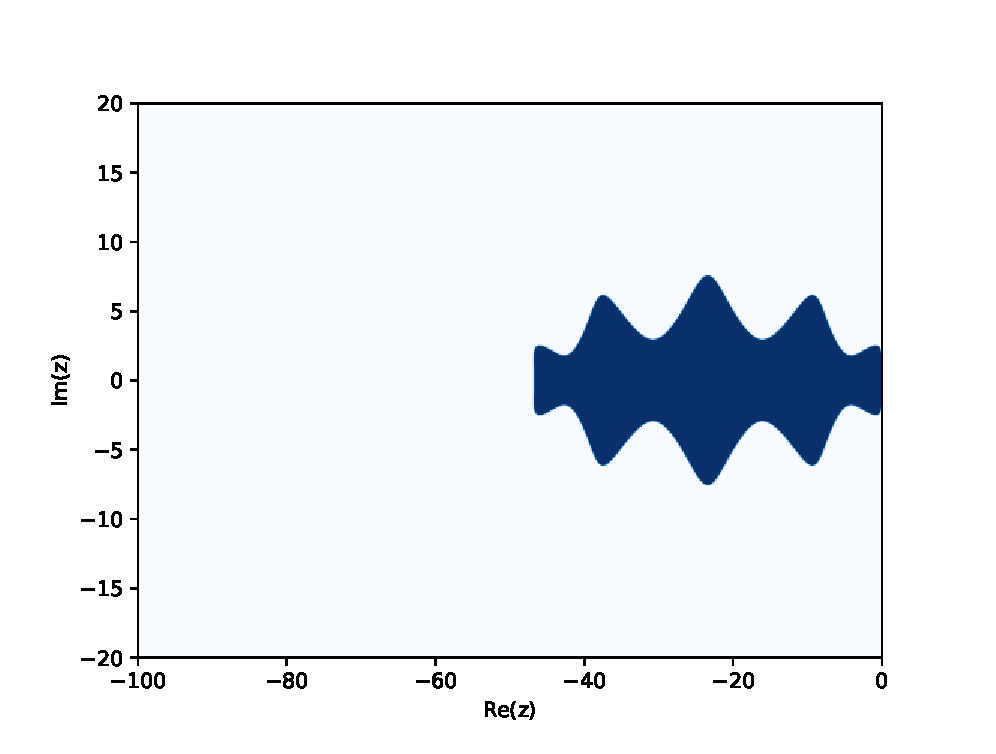
\includegraphics[width=0.3\linewidth]{stable_domians/twostepRKCs10.eps}
    \hfill
    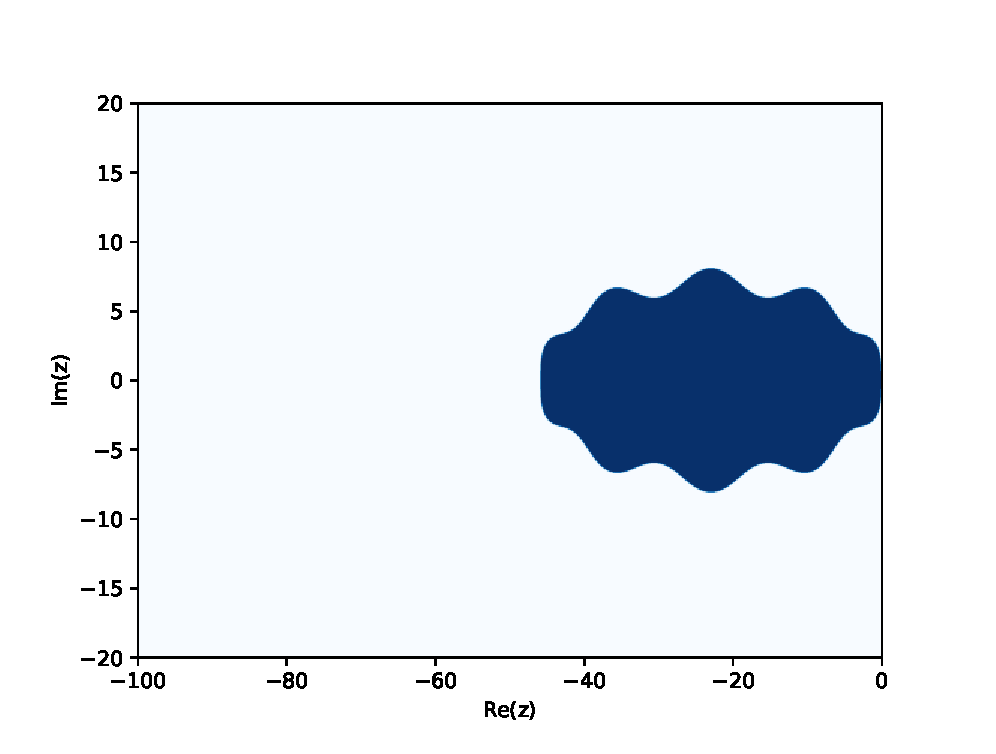
\includegraphics[width=0.3\linewidth]{stable_domians/NTRCKs10wide.eps}
    \hfill
    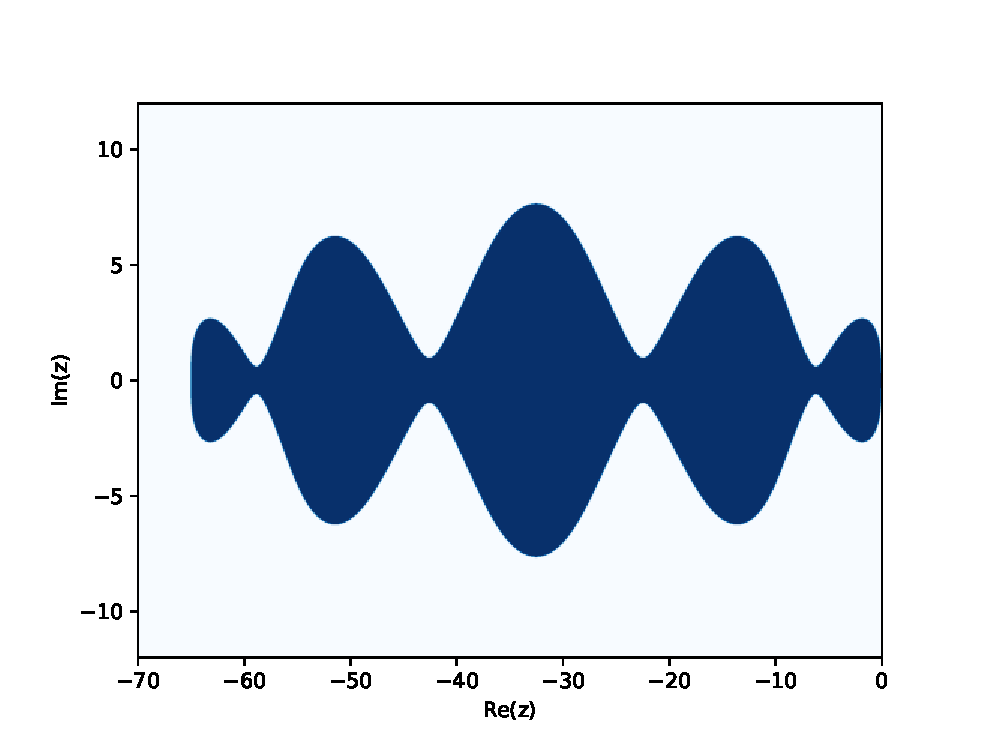
\includegraphics[width=0.3\linewidth]{stable_domians/NTRCKs10long.eps}
    \caption{ Stability domains of method (2.2.1) (left) , NTRKC  with $\varepsilon$ = 4,$\omega_1=\frac{1+\omega_0}{0.45s^2}$ (middle) and  NTRKC  with $\varepsilon$ = 0.05,$\omega_1=\frac{1+\omega_0}{0.65s^2}$ (right) for s=10.}
    \label{fig:1}
\end{figure*}
\begin{figure*}[ht]
    \centering
    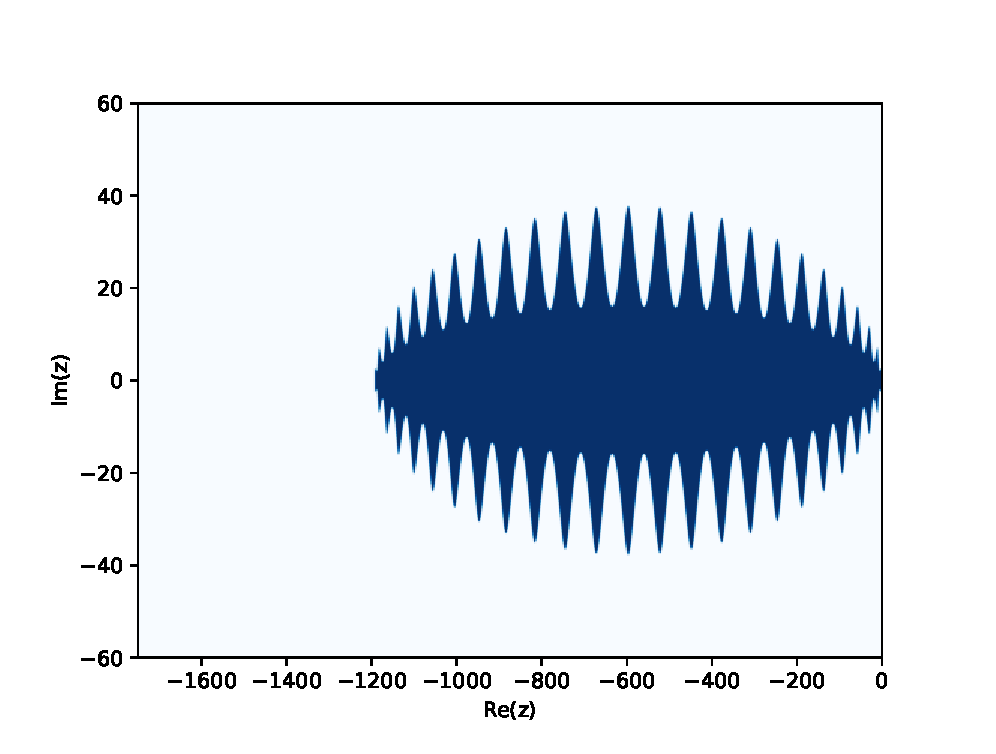
\includegraphics[width=0.3\linewidth]{stable_domians/twostepRKCs50.eps}
    \hfill
    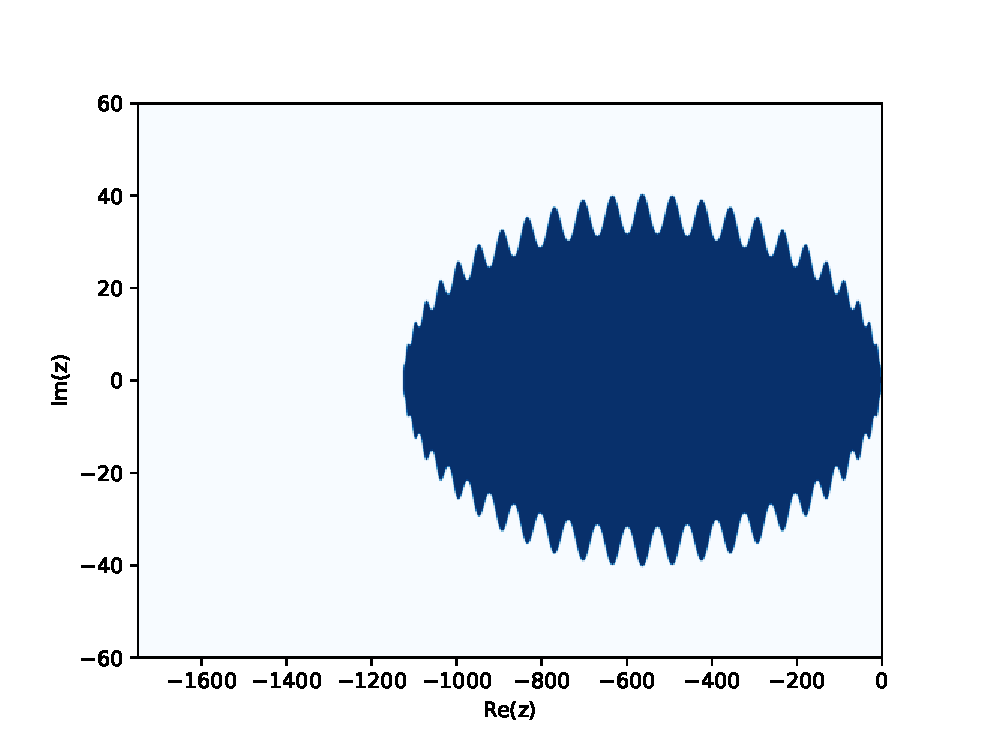
\includegraphics[width=0.3\linewidth]{stable_domians/NTRCKs50wide.eps}
    \hfill
    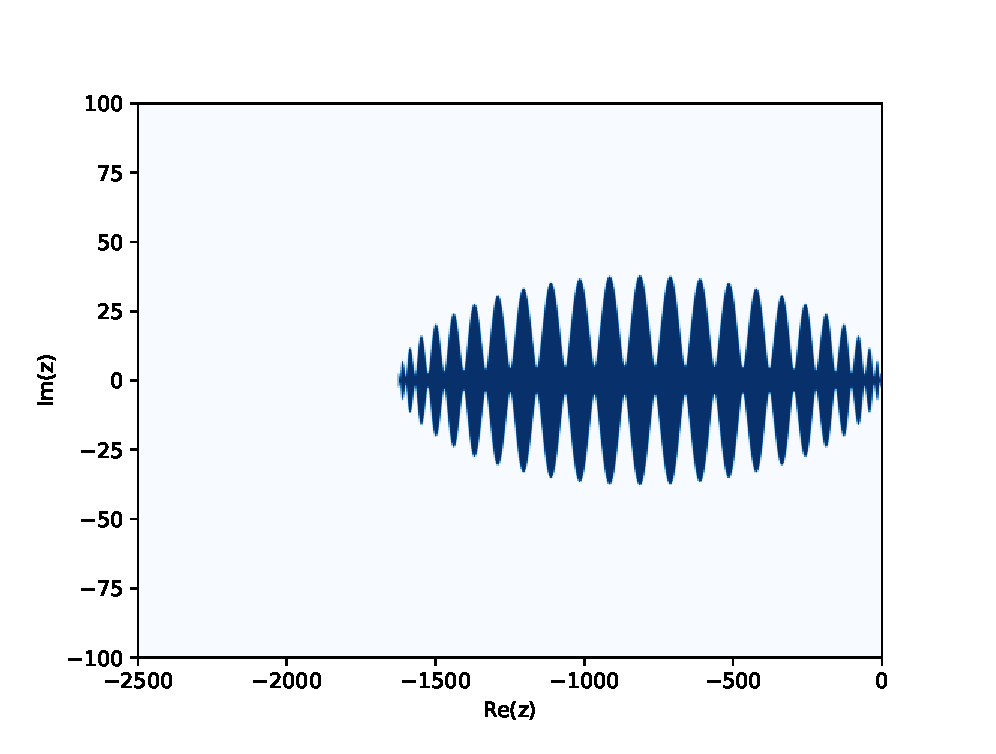
\includegraphics[width=0.3\linewidth]{stable_domians/NTRCKs50long.eps}
    \caption{ Stability domains of method (2.2.1) (left) , NTRKC  with $\varepsilon$ = 4,$\omega_1=\frac{1+\omega_0}{0.45s^2}$ (middle) and  NTRKC  with $\varepsilon$ = 0.05,$\omega_1=\frac{1+\omega_0}{0.65s^2}$ (right) for s=50}
    \label{fig:2}
\end{figure*}
\begin{figure*}[ht]
    \centering
    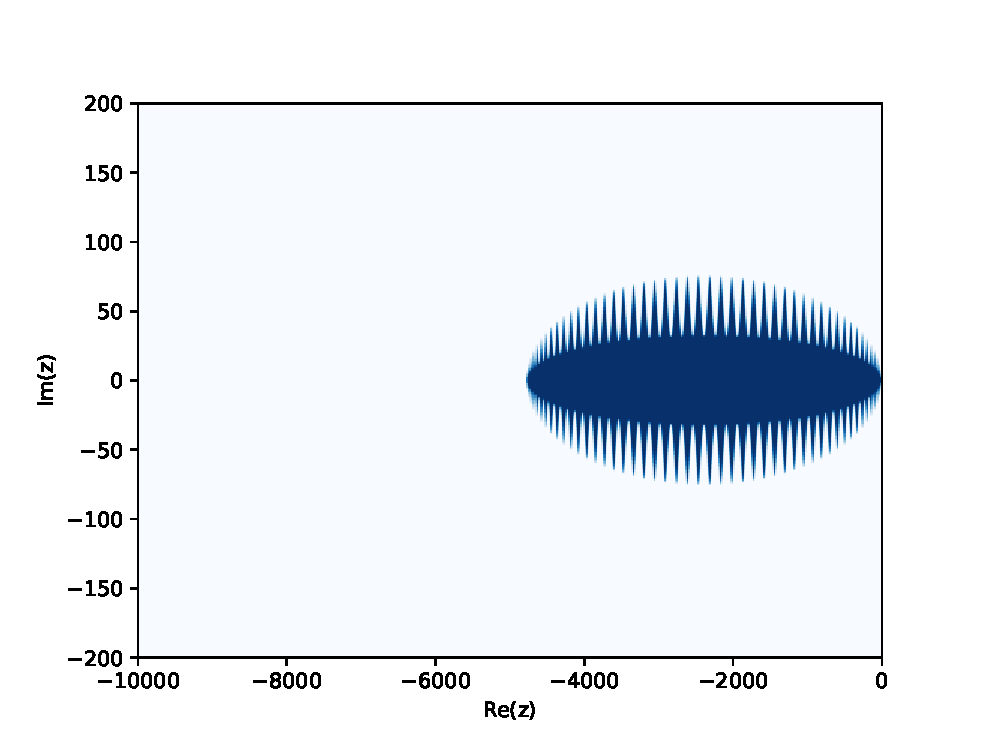
\includegraphics[width=0.3\linewidth]{stable_domians/twostepRKCs100.eps}
    \hfill
    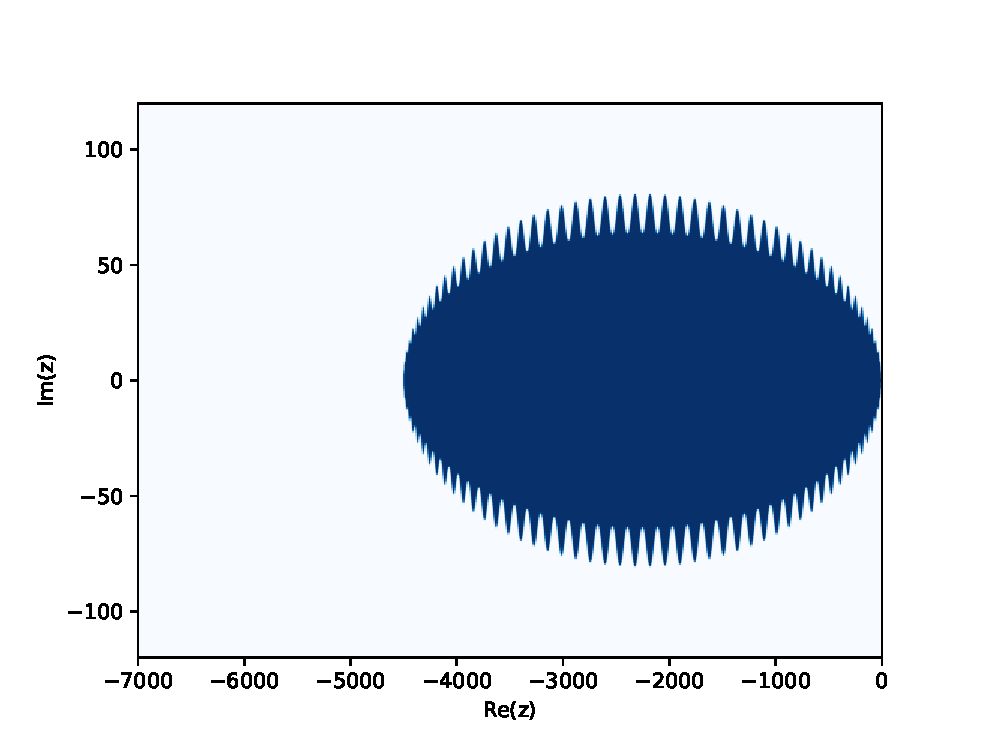
\includegraphics[width=0.3\linewidth]{stable_domians/NTRCKs100wide.eps}
    \hfill
    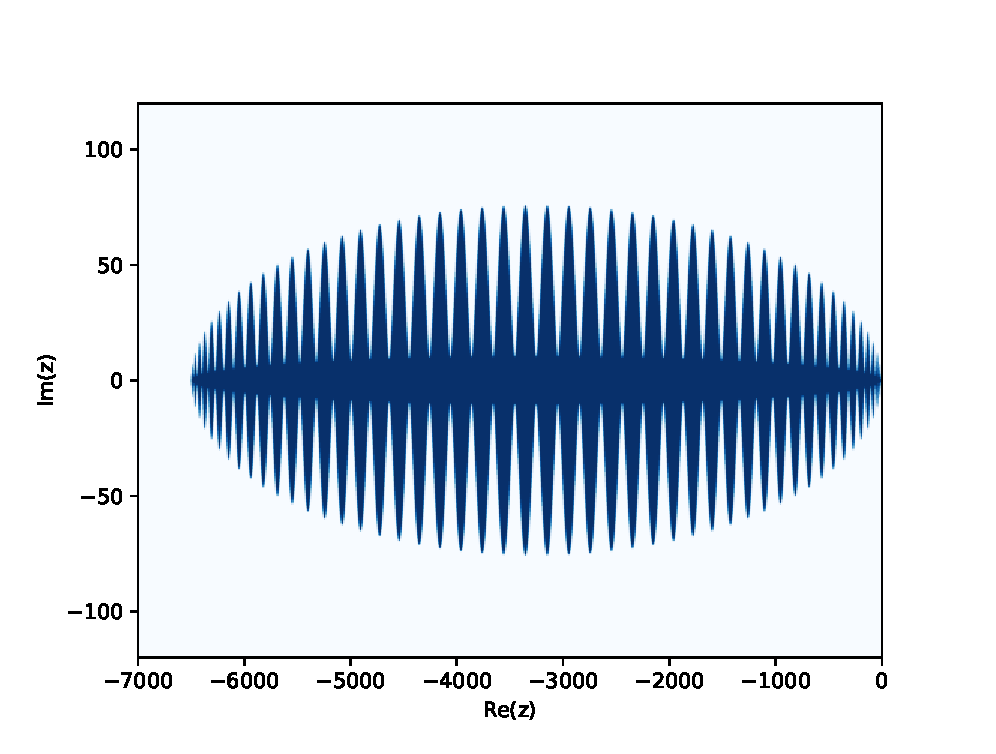
\includegraphics[width=0.3\linewidth]{stable_domians/NTRCKs100long.eps}
    \caption{Stability domains of method (2.2.1) (left) , NTRKC  with $\varepsilon$ = 4,$\omega_1=\frac{1+\omega_0}{0.45s^2}$ (middle) and  NTRKC  with $\varepsilon$ = 0.05,$\omega_1=\frac{1+\omega_0}{0.65s^2}$ (right) for s=50}
    \label{fig:3}
\end{figure*}


When comparing the stability of NTRKC with that of the two-step method,  \figref{fig:1},\figref{fig:2} and \figref{fig:3} clearly illustrate the advantages of NTRKC within the stability domain. Notably, the real boundary of the two-step RKC, denoted as $\tilde{\beta(s)}$, is approximately $0.45s^2$.
 In contrast, NTRKC achieves a real boundary of almost the same magnitude but significantly widens the stability domain in the direction of the imaginary axis. This expansion implies that NTRKC becomes the preferred method when dealing with scenarios involving a large number of Peclet numbers.
Furthermore, it's essential to note that the selection coefficients in equation (3.2.1) come at the expense of the imaginary boundary. The optimal real boundary for the third-order NTRKC, represented as $\beta(s)$, extends up to $0.65s^2$. 
In comparison, the optimal real boundary for the third-order two-step RKC reaches up to $0.45s^2$ (as discussed in [5555]). As a result, NTRKC demonstrates superior performance, particularly in scenarios where diffusion-related problems or diffusion-dominated terms play a crucial role

\section{Variable step strategy }
A series of RKC methods with variable step size [111] is an effective means of solving rigid ordinary differential equations, which can be adapted to different types of rigid problems can significantly improve the speed of computation
\subsection{Error estimate and step size selection}

Numerous investigations have been conducted on the subject of local error estimation, as documented in the literature [19]. 
In this work, we present a local error estimator with a structure akin to the one proposed in a previous study [20]
$$
err_{n+1}=C(12(y_n-y_{n+1})+6\tau(f(y_n)+f(y_{n+1}))),
$$
The weighted RMS norm of the error is defined as
$$
||err_{n+1}||=\sqrt{\frac{1}{d}\sum_{i=1}^d(\frac{err_{i,n+1}}{\emph{tol}})^2},
$$
where \emph{tol} is a permitted tolerance and $\emph{err}_{i,n+1}$ denotes the ith component of $y_{n+1}-\tilde{y}$
(Here, for example,).

There are many choices regarding the size of the new step(see [222]), here we use the step control strategy proposed by jack [999]
$$
\tau_{n+1}=fac\cdot\tau_n\big(\frac{1}{||err_{n+1}||}\big)^{\frac{1}{p}}\frac{\tau_n}{\tau_{n-1}}\big(\frac{||err_n||}{||err_{n+1}||}\big)^{\frac{1}{p}},
$$
where p is the order of consistency and $\emph{fac}=0.8$ is a safety factor,we also  use the traditional control strategy
\begin{align}
  0.1 \le \frac{\tau_n}{\tau_{n+1}} \le 5.\nonumber   
\end{align}
\subsection{Stage number selection}
In a new step of the forward computation, we first chose the step size to control the local error, and then chose minimum stage number such that the stability condition is satisfied
\begin{align}
    \tau\rho(\frac{\partial f}{\partial y}) \le c_ss^2,\nonumber
\end{align}
where $\rho(\frac{\partial f}{\partial y})$ is the spectral radius of the Jacobian matrix $\frac{\partial f}{\partial y}$ and $c_ss^2$ is optimal real stability boundary 
for the above mentioned methods.


Through inequality (4.2.1), we derive the formula for computing stage number s as follows:
\begin{align}
    s=\left\lceil\sqrt{\frac{\tau}{c_s}\rho(\frac{\partial f}{\partial y})}\right\rceil ,\nonumber
\end{align}
For linear ODE systems, the spectral radius is easy to estimate.
For nonlinear systems, we usually use Gershgorin theorem and nonlinear power methods to estimate the spectral radius of the problem.
The nonlinear power method is used in the numerical examples in this thesis

















There are various bibliography styles available. You can select the style of your choice in the preamble of this document. These styles are Elsevier styles based on standard styles like Harvard and Vancouver. Please use Bib\TeX\ to generate your bibliography and include DOIs whenever available.

Here are two sample references: \cite{Feynman1963118,Dirac1953888}

\section*{References}

\bibliography{mybibfile}

\end{document}